\title{CMPS 240 Artificial Intelligence\\RPS-Safari}
\author{Kerui Huang\\khuang7@ucsc.edu}
\date{\today}
\documentclass[10pt]{article}
\usepackage{fullpage}
\usepackage{graphicx}
\usepackage{wrapfig}
\usepackage{bm}
\usepackage{amssymb}
\usepackage{amsmath}
\usepackage{epsfig}
\begin{document}
\maketitle

\section{INTRODUCTION}
Although rock-paper-scissors (RPS) is a very straightforward and simple game, it does involve some fundamental problems about the fields of artificial intelligence, such as how to design a decent algorithm to make the computation of our machine more intelligent. It can be even helpful for us to understand how our intelligence works.

Theoretically, if someone is playing RPS completely randomly, it is impossible to gain any advantage against this player. However, human players tend not to be completely random, neither do most machines. Therefore, after playing a few rounds of RPS against the same opponent, maybe an agent can predict what the opponent will do based on its past experience. In other words, it learns from its experience and changes its behaviors in the future in order to gain an advantage, which makes it intelligent. Therefore, we are interested in finding a computational method, or say an algorithm, for the agent to help it figure out the pattern our opponents have internally. By ``understanding" the opponent, the agent is more likely to win.

\section{STRATEGY}
\subsection{Why Not Random}
Playing randomly is somehow a good strategy. Because it is random, it has no preferences, which means there is no pattern under the hood to be discoved. At this point, it can successfully confuse opponents. 

However, it also means that it is closed, namely, it does not percept anything around it. Therefore, no matter how its opponents play, it does not take their actions into account. But what if an opponent always plays rock? If the agent knows it, it can always play paper to beat this opponent. This strategy is apparently better than playing randomly in this case. The exception is that the opponent plays randomly. But as mentioned above, players are usually non-random. Hence, it is probable to figure out a way to uncover their behaviors.

On the other hand, it is fairly difficult to create an agent that plays completely randomly. In this sense, maybe we can make use of heuristic algorithms to build a strong agent which is more likely to win a tournament involving non-random and predictable competitors.

\subsection{My Strategy}

\subsubsection{Choice}
First, the agent should know \textbf{\textit{which one to play}}. Rock, paper or scissor? Since this is a simple agent (first version), I do not apply complicated computations to this problem. The basic idea is that the agent takes all inputs (the number of rock, paper and scissor played each round), sums them up, and calculate its probability to win by playing rock, paper, scissor respectively. But of course, for the first round, since there is no previous information available, the agent just randomly (more precisely, pseudo-randomly) picks up rock, paper or scissor. Here is a very straightforward example as follows:
\begin{quote}
\textbf{Exmple 1:}\\
Suppose we have ((1 3 4) (8 3 1) (3 4 9)) after 3 rounds. First, the agent takes all the input, and sums them up respectively. Then, the list is flattened as (12 10 14). Therefore, based on this previous experience, the probability \footnote{Maybe not a strict ``probability", but it somehow reflects the probability.} for playing rock, paper and scissor are:
\begin{itemize}
\item R = S - P = 14 - 10 = 4 \footnote{Using the absolute value!!}
\item P = R - S = 12 - 14 = -2
\item S = P - R = 10 - 12 = 2
\end{itemize}
Therefore, playing R is most possible to win, so the agent plays R.
\end{quote}

\subsubsection{Weight}
The second question is \textbf{\textit{how much the agent bets for this round}}. For the first round, the agent just randomly weighs its bet \footnote{In addition, the bet surely cannot break  our RPS-Safari rules. Please see the basic requirements on the website.}. After the first round, the agent knows how it performed in the last round. So here, the idea is to better the weight of its bet according to its past performance named as \textbf{confidence} here. My assumption here is:
\begin{quote}
If the agent played really well in previous rounds, it makes sense that it should be more confident of itself and then bet more than last round, or vice versa.
\end{quote}

Besides this reasonable assumption, some other scenarios should be considered. For example, as Prof. Levinson mentioned in the lecture, even though you wins every time, it is not a good idea to bet all you have. Once you lose, you lose all. Therefore, my considerations are:
\begin{quote}
\begin{itemize}
\item \textbf{Case 1:} When the agent gains a very high score, it is good to be more conservative and thus it can keep its upper hand. ``Conservative" here means it almost keeps its old weight, not increase it dramatically.
\item \textbf{Case 2:} When the agent gains a somewhat high score and it keeps performing very well, and since it has not reach a very high score, it is advisable to let it be more aggressive and consequently adding more weight to its bet so as to make improvements faster.
\item \textbf{Case 3:} When the agent just starts its adventure or it played so far neither too bad nor very well, it had better be conservative and wait until its gain some more experience after some rounds. When it performs better and better (namely, reach case 2), it can begin to bet more.
\item \textbf{Case 4:} So far, I only discussed about the scenarios in which the agent plays just-so-so or well. What if the agent plays very bad? If an agent plays bad, it sort of means that it cannot trust itself. However, it is not all, because it may be helpful as well. If an agent always makes mistakes, next time it can just take the opposite decision. Then, it is very possible for it to gain some points. So, when the agent performs bad, it just reverses its original choice (which is made based on the first three cases).
\end{itemize}
\end{quote}

Then, to formulate these behaviors, my agent utilize the formula \footnote{Note that this formula only can be applied to the cases when the agent plays well. If the agent plays bad, just change the sign of the function.} as follow:
$$
10\times arctan(.05\times (x - 280)) + 16, when\ score\geq 200
$$

The term 280 means the point at which the agent think it should make the fastest improvement. Namely, when the agent reaches 280 points, the increment of the weight is largest. This is an empirical value I gained after some competitions among my agent and random-agents.

The term .05 controls how fast the agent increase the weight of its play. It is still an empirical value.

The term 10 controls the scale of the weight, since the original $arctan$ function is too small to fit our score scale.

The term 16 is used for bounding the absolute value of the weight. Because 
$$
\lim_{x \to -\infty} (10\times arctan(.05\times (x - 280))) = -15.708
$$ and we need to make sure the bet is positive \footnote{Since here we suppose we have positive cases only. For the negative case, we will simply change the sign later.}, we need to add 16 to ensure it is positive.

Figure \ref{figure:a} shows the change of the weight for positive cases.

\begin{figure}
\centering
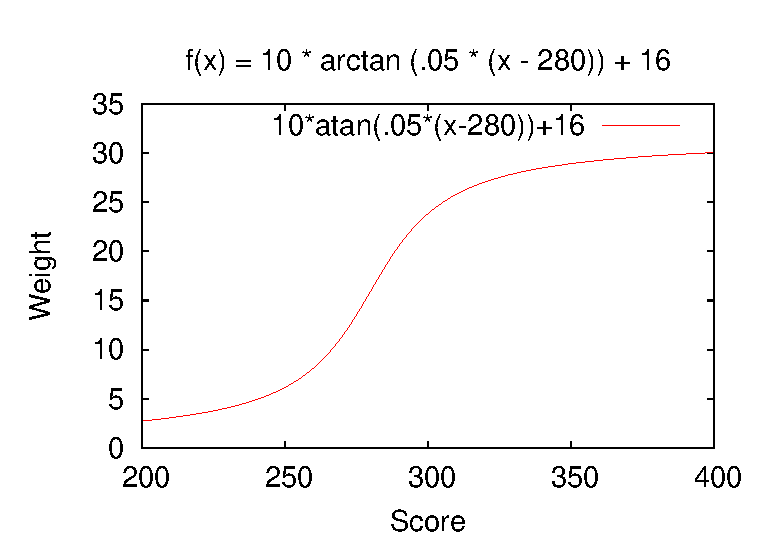
\epsfig{file=a.eps, height=2in, width=2.5in}
\caption{The function $f(x)=10\times arctan(.05\times (x - 280)) + 16, when\ score\geq 200$}
\label{figure:a}
\end{figure}

%\begin{table}
%\caption{Comparing early result rates.($c=\frac{|A||B|M}{(|A|+|B|)^2FT}$)}
%\label{tab:rrcomp}
%\center
%\begin{tabular}{|c|c|} \hline
%& $F=1.2, T_{ri}=T_{wt}=T_{rt}=T$ \\ \hline
%Symmetric Hash & $c$ (Must fit in memory)\\ \hline
%Hash Ripple & $ 0.5c $ \\ \hline
%SMS-Join & $ 0.6c $ \\ \hline
%Block Ripple & $ \frac{2k+1}{k+2}c:c, 1.25c, 1.40c, ... $ \\ \hline
%PR-Join ($ \gamma=1 $) & $ c, 1.7c, 3.2c, 6.2c, 12.2c, ... $ \\ \hline
%\end{tabular}
%\end{table}

%\begin{figure}
%\centering
%\includegraphics[width=50mm]{size.jpeg}
%\caption{A 10G relation joins a 20G relation}
%\label{figure:size}
%\end{figure}
%\bibliographystyle{abbrv}
%\bibliography{bib}
\end{document} 
